%%%%%%%%%%%%%%%%%%%%%%%%%%%%%%%%%%%%%%STARt PREAMBLE
\documentclass{article}

%Required: You must have these
\usepackage{Sweave}
\usepackage{graphicx}
\usepackage{tabularx}
\usepackage{hyperref}
\usepackage{natbib}
\usepackage{pdflscape}
\usepackage{array}
\usepackage{authblk}
\usepackage{gensymb}

%\usepackage[backend=bibtex]{biblatex}
%Strongly recommended
 %put your figures in one place
%\SweaveOpts{prefix.string=figures/, eps=FALSE} 
%you'll want these for pretty captioning
\usepackage[small]{caption}

\setkeys{Gin}{width=0.8\textwidth} %make the figs 50 perc textwidth
\setlength{\captionmargin}{30pt}
\setlength{\abovecaptionskip}{10pt}
\setlength{\belowcaptionskip}{10pt}
% manual for caption http://www.dd.chalmers.se/latex/Docs/PDF/caption.pdf

%Optional: I like to muck with my margins and spacing in ways that LaTeX frowns on
%Here's how to do that
\topmargin -1.5cm  
\oddsidemargin -0.04cm 
\evensidemargin -0.04cm % same as oddsidemargin but for left-hand pages
\textwidth 16.59cm
\textheight 21.94cm 
%\pagestyle{empty}  % Uncomment if don't want page numbers
\parskip 7.2pt   % sets spacing between paragraphs
%\renewcommand{\baselinestretch}{1.5} 	% Uncomment for 1.5 spacing between lines
\parindent 0pt% sets leading space for paragraphs
\usepackage{setspace}
%\doublespacing
\renewcommand{\baselinestretch}{1}
\usepackage{lineno}
 
%%%%%%%%%%%%%%%%%%%%%%%%%%%%%%%%%%%%%%END PREAMBLE 

%Start of the document
\begin{document}

%\SweaveOpts{concordance=FALSE}
\Sconcordance{concordance:bayes4cons_doc.tex:bayes4cons_doc.Rnw:1 310 1}


\bibliographystyle{bibstyles/amnat.bst}
\title{Benefits of Bayesian Modelling For Conservation} 
\author[1,a]{A.K. Ettinger}
\author[2]{H. Eyster}
\author[3]{D. Loughnan}
\author[3]{X. Wang}
\author[3]{E.M. Wolkovich}
\author[3]{M. Auger-Methe}
\author[4]{R. Zenil-Ferguson}
\author[5]{V. Leos Barajas}
\author[6]{Leithen M'Gonigle}
\author[6]{Hanna Jackson}
\author[7]{Others from Symposium working group?}


\affil[1]{The Nature Conservancy,Seattle, Washington, USA}
\affil[2]{TNC}
\affil[3]{UBC}
\affil[4]{UKY}
\affil[5]{University of Toronto}
\affil[6]{SFU}
\affil[7]{Multiple other institutions?}


\affil[a]{Corresponding author; email: ailene.ettinger@tnc.org; mailing address: 74 Wall Street. Seattle, WA 98121, USA }

\date{\today}
\maketitle 
\textbf{Author contributions}: All authors conceived of this manuscript, which began at a Bayesian Generative Modelling Symposium at University of British Columbia in 2024, and all authors contributed to manuscript revisions.

\textbf{Data Accessibility} 

\textbf{Running title} 

\textbf{Key words} 


\textbf{Paper type} Review or Perspective in Frontiers in Ecology and the Environment, Conservation Biology, Conservation Letters, or Conservation Science and Practice

\textbf{Focal Audience} Conservation biologists and other scientists who would like to influence conservation/environmental policy, IPCC 



%%%%%%%%%%%%%%%%%%%%%%%%%%%%%%%%%%%%%%%%%%%%%%%%%%%

%%%%%%%%%%%%%%%%%%%%%%%%%%%%%%%%%%%%%%%%%%%%%%%%%%%

%\linenumbers

\section*{Abstract} 


\newpage
\section* {Introduction: The challenges and needs of today's conservation science are well-suited for Bayesian data analysis}

\par Conservation science in the 21st century seeks to address the dual crises of  climate change and rapid biodiversity loss. These are problems that require urgent action globally, as loss of earth's biodiversity and its benefits are accelerating \citep{brondizio2019assessing, ripple2017extinction,tittensor2014mid}. Conserving biodiversity is the primary motivation for the field of conservation biology \citep{williams2020past} and at the heart of recent international resolutions such as the Convention on Biological Diversity's Aichi targets (UNEP CBD 2010) and of Sustainable Development Goal 15 \citep{assembly2015resolution}. 
\par Climate change brings additional complexity to conservation science, as climate change both affects and is affected by conservation actions. Historically, conservation focused on protecting habitat as a primary strategy, but such approaches are unlikely to be effective for many species, given that many species ranges are shifting with warming (add REFs). In addition, nature conservation has been integrated into global climate change mitigation assessment and efforts, as well, such as through the concept of `natural climate solutions’ (NCS) \citep{Ellis2024}. NCS are intentional human actions (or `NCS pathways') that protect, restore, and improve management of forests, wetlands, grasslands, oceans, and agricultural lands to mitigate climate change \citep{griscom2017natural}.

\par The need for robust and usable conservation science under climate change is necessary at scales ranging from local to global. For example, preserve managers seek guidance about how to best steward nnatural resources for climate resilience (REF), international climate policy relies on scientific data and publications for systematic observation of climate systems and impacts to people. Developing the evidence base for urgent climate and biodiversity questions often requires synthesizing multiple data sources and incomplete datasets, given the complex social ecological systems in which many conservation science problems are grounded. Thus, a critical part of building the evidence base is ensuring reproducibility and transparency,including clear communication of uncertainty \citep{Ellis2024,ipcc2007} 

\par Bayesian data analysis provides a framework and approaches that align well with these needs of conservation science in the 21st century. Bayesian approaches facilitate synthesis of multiple sources of data to update probabilities of focal outcomes of interest after obtaining new data (e.g., priors, see Box 1). Bayesian methods are well-suited to decision making, as they moving beyond strict null-hypothesis testing:
%whereas frequentist inference estimates the probability that the observed data occurred given a particular hypothesis (P(Y|H)),Bayesian inference  
and provide a quantitative measure of the probability of a hypothesis being true given the available data. % (P(H|Y)). Further, Bayesian approaches provide stratightforward approaches to propagate uncertainty through posterior distirbutions. 
Some fields within conservation biology and natural resource management have adopted Bayesian methods (e.g., wildlife mark and recapture models or occupancy models \citep{}, fisheries\citep{}), historically they have not been widely used.

\subsection*{Aim} We aim to highlight features of Bayesian approaches that are well-suited to conservation science, and hope to help accelerate more widespread adoption of Bayesian data analytical approaches in the field, as we believe these approaches could enhance progress, with more  widespread adoption. We show that Bayesian approaches have been steadily increasing in ecology/naturel resource management, highlighting that the time is right for more widespread use in conservation sciences. We describe the benefits of using Bayesian methods for conservation science questions, summarize what is required to use these methods, and provide example code and analyses relevant to current conservation problems. We also share resources and a glossary that we hope will make Bayesian tools more approachable to those who have not used them before.
\section* {Increasing use of Bayesian approaches}
\begin{itemize}
\item Bayesian approaches are increasing in ecology, Fig. \ref{fig:consbaystrend}. variation across fields (more in fisheries, wildlife biology; less in forestry).
\item Bayesian approaches are not standard in approaches globally (IPCC, ) and not widely used in conservation biology, in our experience
%From Lizzie: IUCN `Rules of Procedure’ (download here) are pretty vague on uncertainty (and have two types at least: Uncertainty in the data and uncertainty in taxonomic). I think our relevant interest in the IUCN goal is to get to ‘Direction of current population trend (stable, increasing, decreasing, unknown)’ and there are actually are some papers about what to do about uncertainty in this for the IUCN. One well-cited one is: Making Consistent IUCN Classifications under Uncertainty (2000, JSTOR link), which I think basically advocated fuzzy numbers (but I did not read closely; this paper seems to have led to the RAMAS software). There’s a literature from this citation including a Bayesian network (Use of a Bayesian network for Red Listing under uncertainty, 2010) that someone could dig into a little more? See also: JARA: ‘Just Another Red-List Assessment’
\end{itemize}
\section* {Benefits for Conservation}
\subsection*{Bayesian approaches offer powerful and flexible model that can get the job done!}
\par Ecological data are notoriously poorly aligned with classic stastical techniques (e.g., nonnormal data, unbalanced, etc). This can result in situations where frequentist models are not possible to fit or result in inaccurate interpretations (e.g.,case study 1). Bayesian modelling approaches are flexible and powerful enough to provide robust estimates under a wide range of conditions. 
\par In addition, conservationists are often particularly interested in species with small populations, since these are often the ones most at risk of extinction, or ones that are poorly understood \citep{stinchcombe2002influence}. Frequentist statistics rely on asymptotic behavior, which makes it difficult for these methods to draw useful conclusions from small sample sizes \citep{mcneigh2016using}. Bayesian methods, however, do not have this same reliance, and so are better able to accommodate small sample sizes. However, these methods still require care when working with small sample sizes, because priors matter much more; yet this is also an opportunity to include the full gamut of prior knowledge from many sources that may not typically be included in quantitative analyses \citep{mcneish2016using}. 

\subsection*{Frameworks for integrating multiple data sources}
\par Conservation problems are complex and addressing them, especially in the era of climate change, requires integrating social, economic, biological, and physical information to provide the evidence base upon which decisions can be made. Conservation evidence comes in many forms, including from quantitative studies, community knowledge, expert knowledge, traditional ecological knowledge, and others. Conservation decision-making requires integrating these multiple sources of information to provide an evidence base upon which decisions can be grounded \citep{stern2022interweaving}. Bayesian methods enable two fruitful avenues for such integration. First, information can be amalgamated into Bayesian Belief Networks \citep{marcot2001using,newton2007bayesian}. Second, extant information can be used to inform prior distributions \citep{o2008informed}. 

\subsection*{Adaptive management and comparing alternatives}
\par Conservation scientists often need to compare outcomes from current `business-as-usual' approaches to new alternatives. For example, conservation scientists might be interested in deciding whether an alternative practice produces the same results as current practice. 
The need to test new approaches, coupled with the fact that ecosystems are dynamic and often yield unexpected behaviors \citep{Levin2012,Gross2013}, have led to practices of adaptive management in conservation \citep{holling1978adaptive}. Yet frequentist statistical frameworks rarely provide information necessary to inform adaptive management  \citep{prato2005bayesian}.  Specifically, frequentist statistics incapacity to compare support for a variety of hypotheses \citep[including a `null' hypothesis;][]{Zyl2018} prevents this method from informing what interventions will most likely bring about conservation gains \citep{prato2005bayesian}. For example, in its submission process, leading conservation journal \textit{Conservation Biology} requires that authors recognize that, `8. ensured you have not misinterpreted statistical nonsignificance as no effect if a frequentist approach was used (absence of evidence is not evidence of absence)?' Bayesian analysis, on the other hand, can provide evidence to support a null hypothesis, e.g., that the current and alternative and current management practices produce similar results \citep{gallistel2009importance}.
\subsection*{Ability to quantify and propagate uncertainty} 
\par Bayesian analyses are particularly useful for decision-making because they not only include a range of information types, but also include associated uncertainty \citep{stern2022interweaving}. The integration of multiple datasets required by many conservation problems in turn necessitates quantifying and sometimes propoagating uncertainty across multiple sources and/or multiple modeling steps. Bayesian approaches enable straightforward quantification and  propagation of  uncertainty, including for some conservation problems that can require analyses for which frequentist statistics are unable to compute the associated uncertainties \citep{bolker2009a,bates2006r}. Frequentist statistics produce metrics like confidence intervals and p-values, which have very specific interpretations \citep{fornacon2021bayesian}. However, these metrics are often misinterpreted. Bayesian statistics, in contrast, produces credible intervals, for which the intuitive interpretation matches the technical definition, yielding much more easily interpretable results, particularly for non-statistician colleagues and decision-makers (Fornacon-Wood, 2021). 
\par Moreover, Bayesian methods enable uncertainty to be propagated through multiple analyses, ensuring that end results represent the full uncertainty of the process under study. \citep{draper1995assessment,gilbert2023propagating,Eyster2022,Saunders2019}. For example, using Bayesian methods, one can calculate the abundance of birds in different types of management landscapes such as traditional agriculture and perennial polycultures, and then propagate the uncertainty associated with those abundances into a downstream analysis to test whether the bird communities in the alternative perennial polyculture landscape are maintained simply as an ecological sink \citep{Eyster2022}. 


\par Conservation often requires making easily-interpretable wildlife status categories to inform decision making (Brooks, 2008). For example, conservation might be prioritized for species declining `rapidly' versus `moderately.' These discrete categories require information about when a species' population has passed a particular threshold (Brooks, 2008).  Bayesian models make it possible to assess the evidence for whether a species has surpassed a given threshold (Brooks, 2008). 

\section* {Case Studies}
\subsection*{Robust estimates; bird example (Deirdre, Mao)}
\begin{itemize}

\item Extinction example referenced in \citep{wade2000bayesian}. Compare frequentist (Maximum likelihood) to Bayesian analysis to get at population trend and extinction risk 
\item simulate data
\item insert the text box and figures!
\end{itemize}

\subsection*{Priors; example (Marie)}

\subsection*{Propagating uncertainty; NCS example (Ailene)}
\begin{itemize}
\item Mitigation= flux X extent, Fig. \ref{fig:ncs}
\item uncertainty propogation using posterior
\end{itemize}

\section* {A future with more widespread use of Bayesian modelling in Conservation}
\begin{itemize}
\item Implementing Bayesian modelling is easier than ever before! Computational resources (add some details)- are getting easier and should continue getting easier to develop, test, and refine models that represent focal systems and are able to address relevant questions)
\item Urgency and complexity of problems and systems requires flexible, powerful modelling appraoches 
\item We envision a future in which conservation and ecology students (undegraduate and graduate levels) recieve statistical training to provide strong foundations in Bayesian statistics. Currently the focus of many introductory statistics classes is frequentist methods, which are not appropriate for most ecological data. It doesn't have to be this way! 
\item IPCC and other global institutions should include guidelines for Bayesian approaches increasibly used by ecologists ( Fig. 1), as NCS gets integrated into the climate/biophysical analyses that dominated early IPCC work.
\end{itemize}

\par 
\section* {Box 1: Defining Bayesian Analysis}
Inference in frequentist statistics can take many forms, but here we focus on the most dominant incarnation, which entails testing the significance of a null hypothesis given data, measured with a p-value \citep{Zyl2018}. Bayesian analysis can be formulated in a variety of different ways (Lee, 2011). Frequentist methods have previously dominated ecological analyses
\begin{itemize}

\item Frequentist methods—that rely on the frequency of an event's occurrence in a sample dataset given a particular hypothesis to estimate its probability.
\item Bayesian methods—provides a quantitative measure of the probability that a hypothesis is true using available data
\item Frequentist methods—only make use of the sample data
\item Bayesian methods—bring prior knowledge together with the sample data
\item Frequentist methods—parameters  are considered to be estimates of fixed
\item Bayesian methods—model parameters are treated as random variables
\item Frequentist methods—cares about p-value, significance, confidence interval
\item Bayesian methods—cares about credible interval, prior, posterior
\end{itemize}
Bayesian methods use Bayes Theorem (eqn. 1) to combine our prior knowledge of a system with the available data to estimate the probability of an event. 
Does not assume that parameters are the fixed or true quantities
Since inferences are probabilistic—can perform simulations using the density distributions of their parameters and make stronger inference of models predictive uncertainty
P(A|B) = f(B|A)(A)/P(B)
\par Three components:
\begin{itemize}
\item Posterior distribution (P(A|B)): used to update the prior using the likelihood
\item Likelihood ( f(B|A)): function of how likely te response variable is given the data
\item Prior ((A)): pre-existing information about the hypothesis—data from pilot studies or previous experiments, knowledge from experts or the literature—reflect the uncertainty within the system
\end{itemize}
\par Bayesian modeling is an iterative process: analyses may start with insufficient knowledge and data but use experiments to inform priors, and uses model checking to test key assumptions and our understanding of the data generating process.
\par General bayesian workflow 
\begin{itemize}
\item Simulate data based on priors and initial model specification 
\item Collect data
\item Model construction and testing
\item Prior predictive checks→Fit model to data
\item Posterior predictive checks
\item Summarize posteriors
\item Report results to targeted audiences
\end{itemize}



\section* {Box 2: Resources to Get Started}
\underline{Priors}
\par Default priors. Chosen without critical thought or evaluation. Fear ob being too subjective. Defending prior choice promotes good statistical inference
\par Resources on priors: 

\begin{itemize}
\item Banner et al. 2020 https://besjournals.onlinelibrary.wiley.com/doi/full/10.1111/2041-210X.13407 
\end{itemize}

\par Resources on model checking:
\begin{itemize}
\item Conn et al. 2018 %https://esajournals.onlinelibrary.wiley.com/doi/full/10.1002/ecm.1314?casa_token=xI6HXgrOhMAAAAAA%3AkQL_00kjFJjSqOi_iAejxbimMaXP5Gy6kdFPUjVAyzxzLA9KLdzgkl91DM7-XbT1PFxiqZdievS5fro
\item Gentle Introduction to Bayesian statistics (van de Schoot et al. 2014)
https://www.ncbi.nlm.nih.gov/pmc/articles/PMC4158865/
\item Bayesian model selection for ecologists. Hooten and Hobbs 2015
 https://doi.org/10.1890/14-0661.1
\item Bayesian Inference for ecologists. Ellison 2004
 https://doi.org/10.1111/j.1461-0248.2004.00603.x
\item Why becoming Bayesian? Clark 2004
 https://doi.org/10.1111/j.1461-0248.2004.00702.x

\end{itemize}
 

\bibliography{conslib.bib}

\section* {Figures}

\begin{figure}[h]
\centering
 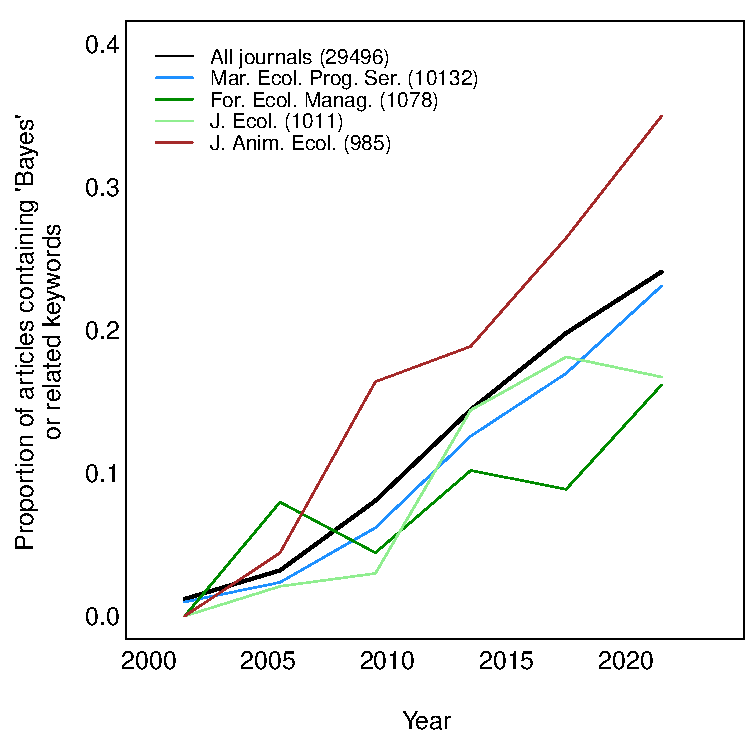
\includegraphics{../figs/conservation.pdf}
 \caption{\textbf{Proportion papers using Bayes in XX major conservation journals since 2000}} 
 \label{fig:consbaystrend}
 \end{figure}
 
 \begin{figure}[h]
\centering
 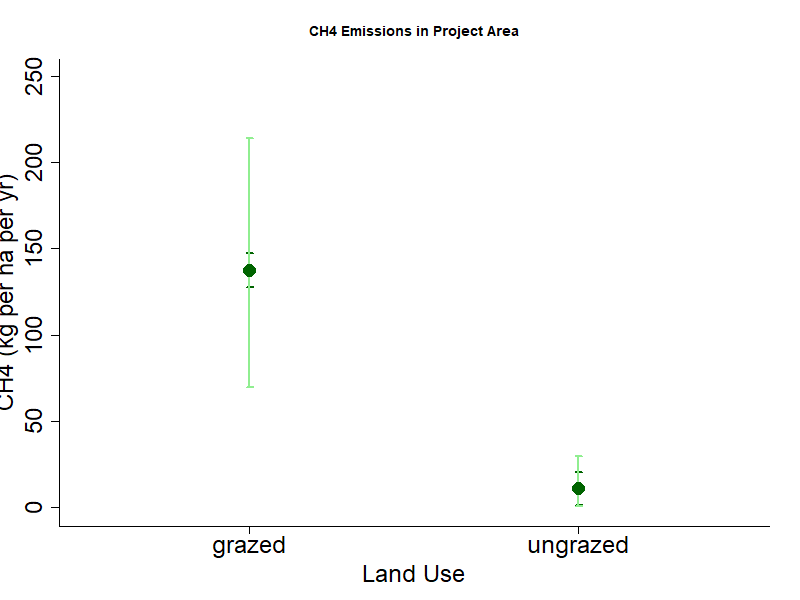
\includegraphics{../figs/ncs/ncsprojimpactch4.png}
 \caption{\textbf{NCS Example: Uncertainty propagation}} 
 \label{fig:ncs}
 \end{figure}
%%%%%%%%%%%%%%%%%%
%%%%%%%%%%%%%%%%%%%%%%
\end{document}
%%%%%%%%%%%%%%%%%%%%%%%%%%%%%%%%%%%%%%%%
% and for Nationally Determined Contributions, National Adaptation Plans, and other climate plans within the United Nations climate process are informed by the 'best available science.'
%Questions for the group:
%1) How detailed to get in Bayesian methods/theory in introduction?
